% Overleaf-ready note: Camera-settings factorial and exposure policy for D65-FairFace7-ROI
% Upload to Overleaf (pdfLaTeX). Optional figures (same folder as this .tex):
%   de00_by_setting_letter.png
%   de00_vs_shutter.png
%   de00_vs_iso.png
%   Lstar_vs_settings.png
% from results/camera_settings/
%
% Pinned numbers:
%   results/camera_settings/summary.json
%   results/pansor20_exposure_audit/summary.json
%   results/pansor20_exposure_residual/summary.json
%   results/pansor20_fairface7/summary.json
%   results/pansor20_fairface7/honesty_check/summary.json
% Code: scripts/evaluate_camera_settings.py, scripts/audit_pansor_exposure.py,
%       scripts/fit_exposure_residual.py, scripts/dng_exif.py
%
% Compile: pdflatex camera_settings_exposure_overleaf.tex

\documentclass[11pt]{article}

\usepackage[margin=1in]{geometry}
\usepackage{booktabs}
\usepackage{siunitx}
\usepackage{amsmath,amssymb}
\usepackage{graphicx}
\usepackage[hidelinks]{hyperref}
\usepackage{enumitem}
\usepackage{xcolor}

\sisetup{
  round-mode=places,
  round-precision=2,
  detect-weight=true,
  detect-family=true,
}

\newcommand{\deee}{\ensuremath{\Delta E_{00}}}
\newcommand{\pipename}{\texttt{D65-FairFace7-ROI}}
\newcommand{\EV}{\mathrm{EV}_{\mathrm{proxy}}}

\title{Camera Exposure and Chart-Free Skin Colorimetry:\\
  ISO/Shutter Factorial, Pansor Audit, and Capture Policy}
\author{FitSkin / Pansor, Camera Settings Dataset}
\date{August 2026}

\begin{document}
\maketitle

\begin{abstract}
We study how iPhone ProRAW camera settings affect chart free flash/no flash cheek CIELAB under the frozen \pipename{} stack.
On a controlled Camera Settings Dataset ($N=95$ aligned A to H captures, four participants with FitSkin Inside Lab), $\deee$ is strongly tied to absolute exposure: $\mathrm{corr}(\deee,\log_2(\mathrm{ISO}\cdot t))$ is about \num{0.78}.
Preferred cells (ISO about 95, shutter about $1/250$ to $1/120$\,s) achieve mean $\deee$ about \num{3} to \num{5}. Long shutter (about $1/60$\,s) or ISO$\ge$200 inflate pipeline $L^*$ into the 78 to 85 range and raise mean $\deee$ to about 15 to 21.
An EXIF audit of the Pansor-20 indoor cohort ($N=65$) shows that production captures are already fully in band (ISO 50 to 125, shutter always $1/120$\,s, mean $\deee=\num{3.63}$ with FairFace-7 ROI).
A leave one person out exposure residual fitted on the factorial improves camera settings LOO $\deee$ but \emph{does not transfer} to Pansor (especially Black participants) and must not enter the color path.
Person specific ROI patches that push Pansor toward $\deee$ about $2.7$ overfit named subjects. A 15/5 threshold retune check and a cheek tone to ethnicity router both favor keeping the published FairFace-7 defaults at $\deee=\num{3.63}$.
We recommend locking AE near ISO 64 to 100 and $1/120$ to $1/250$\,s, with a reject or re prompt gate for ISO$\ge$200, shutter$\ge 1/60$\,s, or cheek $L^*$ above about 75.
\end{abstract}

\tableofcontents
\newpage

%=============================================================================
\section{Motivation}
%=============================================================================

The deployment stack \pipename{} recovers cheek CIELAB under D65 from indoor iPhone flash/no flash ProRAW without an in scene ColorChecker, using a frozen colorimetric path and FairFace-7 routed cheek sampling \cite{d65fairface7note}.
On Pansor-20 it achieves mean $\deee=\num{3.63}$ (median \num{3.44}).
That number assumes captures already sit in a benign exposure regime.
This note asks four practical questions:

\begin{enumerate}[leftmargin=*,itemsep=2pt]
  \item How sensitive is the frozen path to deliberate ISO and shutter changes?
  \item Are current Pansor app captures already in a safe band?
  \item Should an exposure residual learned on a settings factorial be folded into the Lab pipeline?
  \item After exposure is controlled, should further person tuned ROI patches or a tone to ethnicity classifier replace FairFace-7?
\end{enumerate}

%=============================================================================
\section{Methods}
%=============================================================================

\subsection{Color path (frozen)}
All camera settings $\deee$ values use the claimable colorimetric path of \pipename{}:
pre AWB demosaic $\to$ flash/no flash cheek median exposure match $\to$
$\mathbf{R}=\sqrt{\mathbf{A}\odot\mathbf{B}}$ $\to$ pooled $3{\times}4$ affine
(\texttt{tier3\_affine}) $\to$ Bradford CAT from a fixed 5500\,K Planckian white to D65
$\to$ trimmed mean cheek Lab (\texttt{l-sampling off}).
Pansor-20 headline numbers additionally enable FairFace-7 cheek ROI sampling
(\texttt{--l-sampling fairface7}). That ROI layer is a heuristic router, not part of the colorimetric model.
The demosaic/affine/CAT stack is \emph{not} modified in this study.

\subsection{Camera Settings Dataset}
Captures were collected through the Pansor app as flash/no flash ProRAW zips (same layout as Pansor indoor: \texttt{1\_raw\_Photo.dng}, \texttt{2\_raw\_RAW\_\_\_Flash.dng}, Apple landmark JSON).
Nominal shutter, ISO, and white balance (6496\,K) per setting letter came from \texttt{Camera Settings Aug10.xlsx}. FitSkin Inside Lab footer values provided ground truth.

\begin{table}[t]
\centering
\caption{Subjects in the Camera Settings Dataset.}
\label{tab:subjects}
\begin{tabular}{@{}llccc@{}}
\toprule
Person & FitSkin $(L^*,a^*,b^*)$ & Settings & $N$ zips & Notes \\
\midrule
Giana  & $(60.49,\,12.49,\,16.98)$ & A to H & 25 &  \\
Keaton & $(59.43,\,14.92,\,13.62)$ & A to H & 25 &  \\
Parker & $(55.81,\,11.36,\,22.12)$ & A to H & 22 & missing E1 \\
Wooj   & $(58.51,\,13.29,\,20.66)$ & A to H & 23 & Woojae. exclude letter I \\
\bottomrule
\end{tabular}
\end{table}

\paragraph{Factorial design.}
Letters A to D sweep shutter at roughly fixed ISO. Letters E to H sweep ISO at roughly fixed shutter.
All four people share this A to H grid, so setting comparisons line up across subjects.
White balance was locked at 6496\,K in the spreadsheet plan.
Wooj (spreadsheet sheet \texttt{Woojae}) also had a letter I cell (ISO 111 at $1/127$\,s), a near repeat of the baseline ISO band. We exclude I from cross person tables and figures so A to H stay aligned.
\texttt{Wooj2.zip} was excluded as unparsed.
Reported $N=95$ successful A to H trials.

\subsection{Exposure proxy}
Define a relative exposure proxy from no flash EXIF (or spreadsheet nominals on the factorial):
\begin{equation}
  \EV = \log_2(\mathrm{ISO}\cdot t),
\end{equation}
where $t$ is ExposureTime in seconds.
Overexposure in this note means large $\EV$ and/or inflated pipeline cheek $L^*$ (typically above about 75 to 80), not a sensor white level fraction (though WhiteLevel$=4095$ is available in the DNGs).

\subsection{Pansor-20 exposure audit}
For each of the $N=65$ indoor FairFace7 evaluation trials, we read no flash DNG EXIF (ISO, ExposureTime, WhiteBalance) via TIFF IFDs and joined them to pipeline $L^*$ and $\deee$ from \texttt{pansor20\_fairface7}.
Out of band flags: ISO$\ge$200, shutter$\ge 1/60$\,s, or pipeline $L^*\ge 75$.

\subsection{Exposure residual (post Lab, experimental)}
On camera settings trials we fit ridge residuals predicting FitSkin Lab minus pipeline Lab from features of $\EV$ and pipeline Lab (or full Lab).
Leave one person out (LOO) over \{Giana, Keaton, Parker, Wooj\} selects between an $L^*$ only residual and a 3D Lab residual.
The selected model is then applied as a \emph{post Lab} correction on Pansor-20.
Per protocol: a Pansor ``win'' is claimed only if (i) LOO improves on camera settings \emph{and} (ii) Pansor mean $\deee$ decreases.
Otherwise the frozen path is left unchanged.

\subsection{ROI honesty checks (non exposure)}
After confirming Pansor is exposure in band, remaining error is ROI/sampling dominated.
We reject person specific ROI patches (Latino to Indian remaps, White high $a^*$ rejects, Black $b^*$ gated chroma boosts) that can push cohort mean $\deee$ toward about $2.7$ but fire on named subjects.
Two cheap checks support keeping published FairFace-7 defaults:
\begin{itemize}[leftmargin=*,itemsep=2pt]
  \item \textbf{15/5 threshold retune:} 40 random splits. Coordinate descent retune of ROI thresholds on 15 people, score the held out 5.
  \item \textbf{Tone to ethnicity LOSO:} logistic regression on cheek $L^*,a^*,b^*,C^*$, ITA, $L$ percentiles predicts the ROI ethnicity key without FairFace.
\end{itemize}

%=============================================================================
\section{Results}
%=============================================================================

\subsection{Camera settings factorial}

\begin{table}[t]
\centering
\caption{Mean frozen path $\deee$ and pipeline cheek $L^*$ by setting letter ($N=95$, A to H only).
Rows follow the design order so shutter and ISO sweeps line up across people.}
\label{tab:settings}
\begin{tabular}{@{}lrrrrr@{}}
\toprule
Letter & Role & Median shutter & Median ISO & Mean $\deee$ & Mean $L^*$ \\
\midrule
A & shutter baseline & about $1/130$\,s & about 103 & \num{4.63} & \num{62.64} \\
B & shutter long & about $1/60$\,s & 95 & \num{18.63} & \num{81.75} \\
C & shutter faster & about $1/250$\,s & 95 & \num{5.42} & \num{53.40} \\
D & shutter fastest & about $1/500$\,s & about 103 & \num{7.31} & \num{51.17} \\
E & ISO baseline & about $1/130$\,s & 95 & \num{3.40} & \num{58.15} \\
F & ISO 200 & about $1/130$\,s & 202 & \num{15.65} & \num{77.67} \\
G & ISO about 400 & about $1/130$\,s & about 398 & \num{21.17} & \num{85.29} \\
H & ISO about 1600 & about $1/130$\,s & about 1604 & \num{20.19} & \num{83.86} \\
\bottomrule
\end{tabular}
\end{table}

Overall mean $\deee=\num{12.41}$ (median \num{14.04}) across A to H, dominated by deliberately bad exposures.
Across trials, $\mathrm{corr}(\deee,\EV)$ is about \num{0.78} and $\mathrm{corr}(L^*,\EV)$ is about \num{0.87}.
E to H ISO values match across people (95 / 202 / about 400 / about 1600).
A to D shutters match (about $1/130$, $1/60$, $1/250$, $1/500$\,s). ISO on A to D is 95 for Giana/Keaton and 111 to 116 for Parker/Wooj, so A is not always identical to E.
The pattern is consistent across all four photographed subjects: preferred cells stay near the Pansor FairFace7 baseline ($\deee$ about \num{3.63}). Overexposed cells fail primarily through $L^*$ inflation rather than ethnicity specific chroma quirks.

\begin{figure}[t]
\centering
% Upload de00_by_setting_letter.png from results/camera_settings/
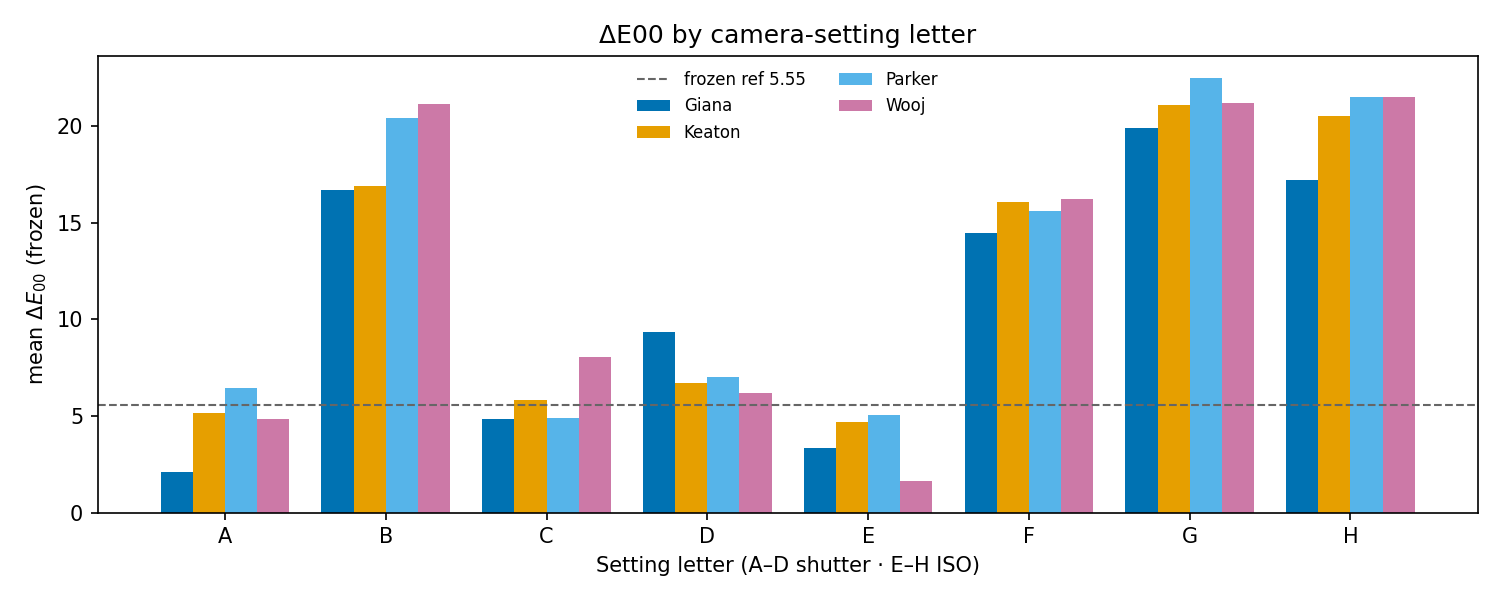
\includegraphics[width=0.92\linewidth]{de00_by_setting_letter.png}
\caption{Mean frozen $\deee$ by setting letter for Giana, Keaton, Parker, and Wooj.
Dashed line: frozen trimmed mean Pansor reference ($\deee=\num{5.55}$). FairFace-7 cohort mean is $\deee=\num{3.63}$.}
\label{fig:byletter}
\end{figure}

\begin{figure}[t]
\centering
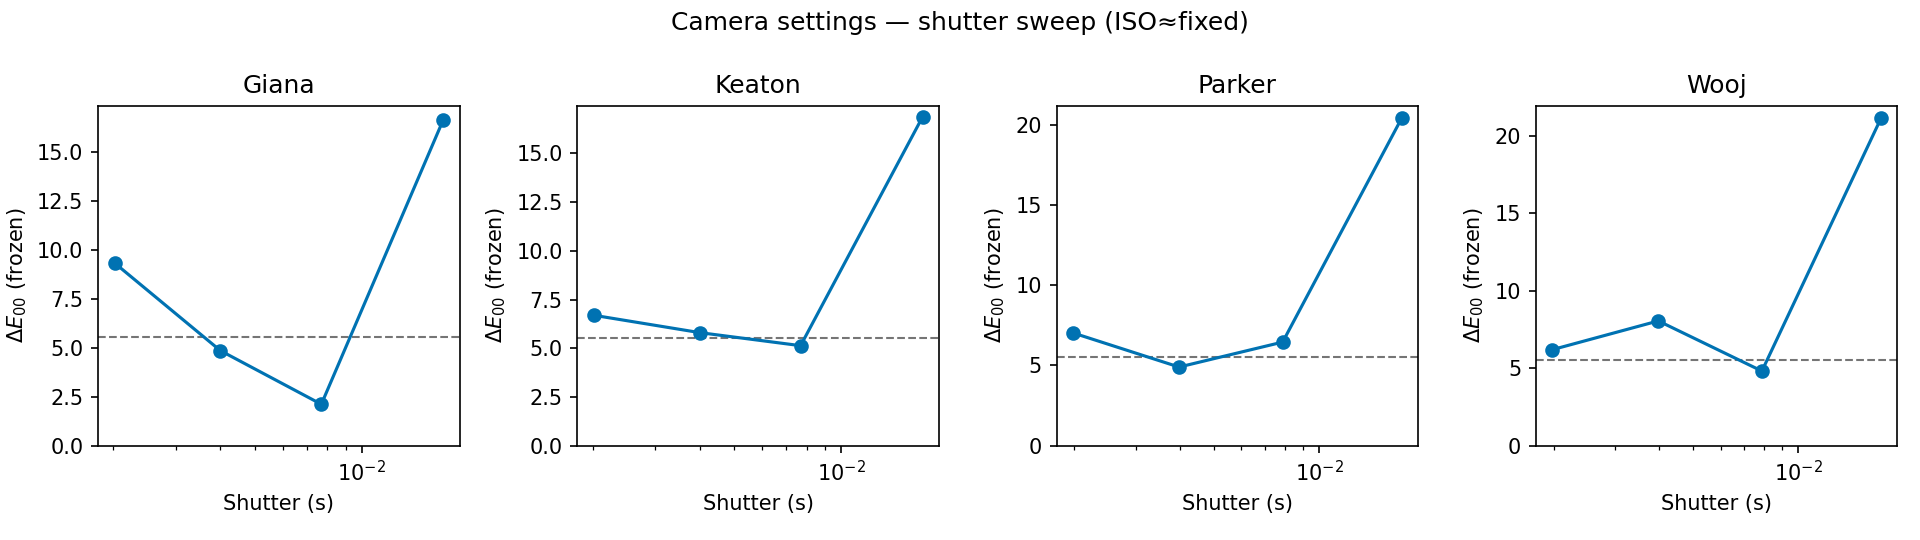
\includegraphics[width=0.92\linewidth]{de00_vs_shutter.png}
\caption{Shutter sweep (ISO roughly fixed): $\deee$ vs.\ ExposureTime.
Long shutter (about $1/60$\,s, cell B) is catastrophic for every subject.}
\label{fig:shutter}
\end{figure}

\begin{figure}[t]
\centering
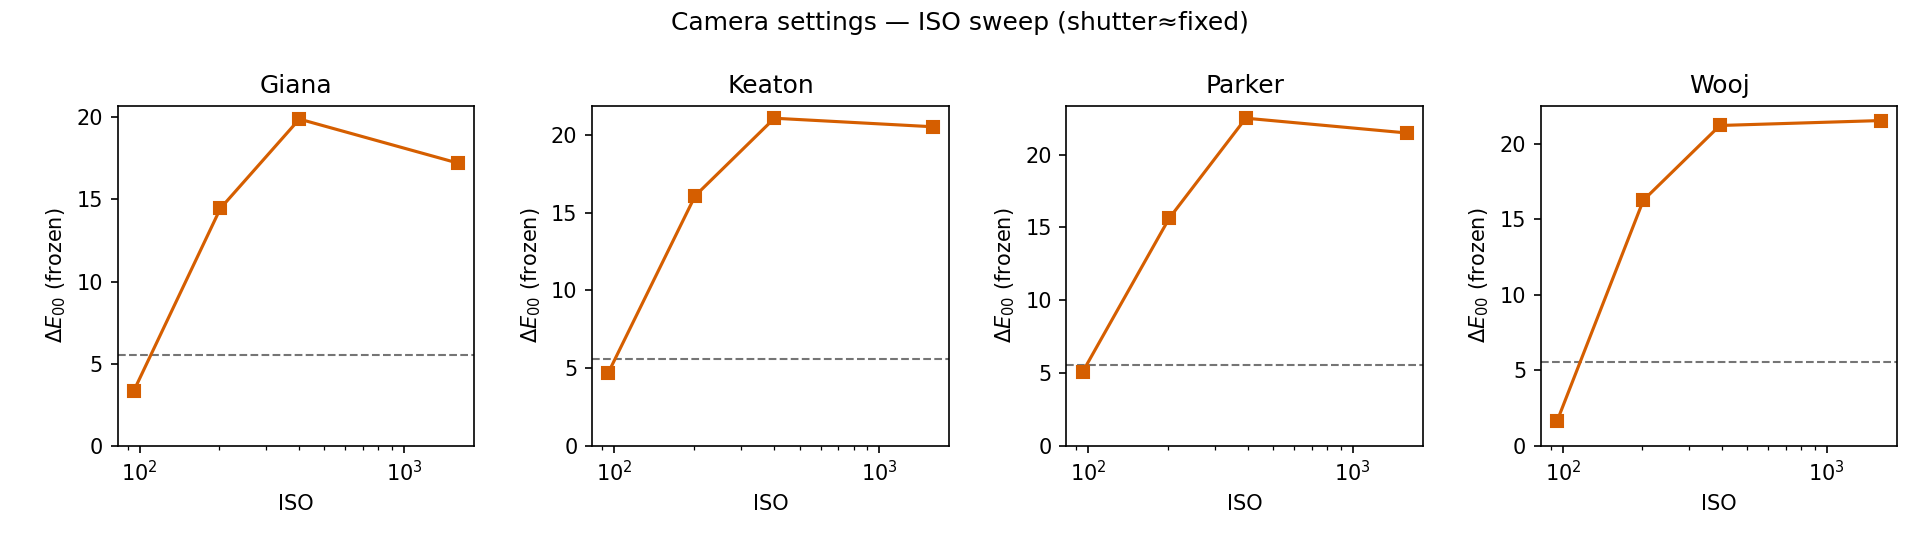
\includegraphics[width=0.92\linewidth]{de00_vs_iso.png}
\caption{ISO sweep (shutter roughly fixed): $\deee$ vs.\ ISO.
ISO$\ge$200 (cells F to H) drives mean $\deee$ into the mid teens to twenties.}
\label{fig:iso}
\end{figure}

\subsection{Pansor-20 already in band}

\begin{table}[t]
\centering
\caption{No flash EXIF audit of the Pansor-20 FairFace7 indoor set ($N=65$).}
\label{tab:audit}
\begin{tabular}{@{}lr@{}}
\toprule
Quantity & Value \\
\midrule
ISO range (min / median / max) & 50 / 64 / 125 \\
Shutter & always $1/120$\,s \\
Pipeline $L^*$ max & about \num{66.6} \\
Flags: ISO$\ge$200 & 0 \\
Flags: shutter$\ge 1/60$\,s & 0 \\
Flags: $L^*\ge 75$ & 0 \\
In band fraction & \num{1.00} \\
Mean / median $\deee$ (FairFace7) & \num{3.63} / \num{3.44} \\
\bottomrule
\end{tabular}
\end{table}

Production Pansor indoor captures already sit in the preferred exposure band.
A simple reject overexposed gate therefore cannot improve the current Pansor headline $\deee$. Its value is prospective (future collections, outdoor / dark rooms, AE drift).

\subsection{Exposure residual: helps factorial, hurts Pansor}

\begin{table}[t]
\centering
\caption{Leave one person out on camera settings and transfer to Pansor-20.
``In band'' = ISO$<$200, shutter$< 1/60$\,s, pipeline $L^*<$75 ($n=49$, includes Wooj I).}
\label{tab:residual}
\begin{tabular}{@{}lccc@{}}
\toprule
Evaluation & Uncorrected mean $\deee$ & Best residual & Mean $\deee$ \\
\midrule
Camera settings LOO (all cells) & \num{12.09} & Lab residual & \num{3.19} \\
Camera settings LOO (in band) & \num{5.17} & $L^*$ residual & \num{2.87} \\
Pansor-20 (selected in band $L^*$) & \num{3.63} & $L^*$ residual & \num{7.40} \\
\quad Black stratum ($n=14$) & \num{3.34} & $L^*$ residual & \num{17.97} \\
\quad Iranian stratum ($n=6$) & \num{3.47} & $L^*$ residual & \num{2.32} \\
\bottomrule
\end{tabular}
\end{table}

LOO on the factorial is a clear win because many cells are severely overexposed and a residual can pull $L^*$ back toward FitSkin.
Transfer to Pansor fails: the four camera settings subjects are relatively light skinned, and the residual systematically harms darker Pansor participants (Black mean $\deee$ rises from \num{3.34} to \num{17.97}).
\textbf{No Pansor win is claimed.} The residual must not be integrated into the deployment color path.

\subsection{Non exposure residual: keep FairFace-7 defaults}
\label{sec:roi-honesty}
Because Pansor-20 is already exposure in band, further gains would have to come from ROI sampling.
Person specific gates (e.g.\ Latino to Indian for Utsav like cheeks) can reduce cohort mean $\deee$ from \num{3.63} toward about $2.7$ to $3.3$, but they are cohort overfit and are \textbf{not} part of the published stack.

\begin{table}[t]
\centering
\caption{ROI threshold honesty check and tone to ethnicity alternative on Pansor-20 ($N=65$).
Frozen $=$ published \pipename{} FairFace-7 defaults.}
\label{tab:honesty}
\begin{tabular}{@{}lcc@{}}
\toprule
Protocol & Mean $\deee$ & Notes \\
\midrule
Full cohort, frozen FairFace-7 ROI & 3.63 & Headline \\
Holdout 5, frozen (40$\times$ 15/5 splits) & $3.70\pm0.55$ & p10 to p90: 3.00 to 4.49 \\
Retune thresholds on 15 $\to$ test on 5 & train 3.34 / test 3.88 & Retune wins 38\% of splits \\
LOSO threshold retune (person means) & frozen 3.69 / retune 3.88 & $\Delta{+}0.19$ \\
Tone to ethnicity + ROI (LOSO) & 3.89 & Weaker than FairFace \\
Demographics ethnicity + ROI (oracle) & 3.23 & Upper bound only \\
\bottomrule
\end{tabular}
\end{table}

Retuning ROI thresholds on 15 people looks good on the train fold but \textbf{worsens} held out error on average.
A cheek tone to ethnicity classifier (LOSO) is also weaker than FairFace-7 ($\deee=\num{3.89}$ vs.\ $\num{3.63}$, ethnicity accuracy about $52\%$).

\paragraph{Ambiguous appearances (Charles, Yuan, Jalona).}
Tone based race routing does not help these cases:
\begin{itemize}[leftmargin=*,itemsep=2pt]
  \item \textbf{Charles} (Asian): FairFace$\to$Asian, tone LOSO$\to$Indian. $\deee$ unchanged ($4.24$), because both keys hit the same low $a^*$ shadow/hiC branch.
  \item \textbf{Yuan} (Asian): FairFace$\to$Asian, tone$\to$Iranian/White. $\deee$ rises $2.68\to4.81$.
  \item \textbf{Jalona} (Black, lighter / higher chroma than other Black subjects): FairFace$\to$Black (correct $L_{p10}$), tone$\to$Indian. $\deee$ rises $2.99\to4.99$.
\end{itemize}
\textbf{Recommendation:} keep FairFace-7 as the ROI prior. Do not weld person specific gates or tone to ethnicity into the claimable stack.
If tone is used later, it should gate sampling features directly ($L^*$/$C^*$/ITA), not predict another race label.

%=============================================================================
\section{Capture policy for the Pansor app}
%=============================================================================

\begin{itemize}[leftmargin=*]
  \item \textbf{Preferred AE band:} ISO $\le$100 and shutter $\in[1/250,\,1/120]$\,s (cells A/C/E).
  \item \textbf{Reject or re prompt:} ISO$\ge$200, shutter$\ge 1/60$\,s, or estimated cheek $L^*$ above about 75 after the frozen path.
  \item \textbf{Do not} apply a post Lab exposure residual trained only on the current four person factorial.
  \item \textbf{Do not} apply person specific ROI patches or tone to ethnicity in place of FairFace-7 for headline claims.
  \item Keep \pipename{} (frozen color + FairFace-7 ROI) unchanged for Pansor-20 reporting at mean $\deee=\num{3.63}$.
\end{itemize}

Relative flash/no flash median matching and per frame 99.5th percentile normalization do \emph{not} rescue absolute overexposure: they equalize the pair and stretch dynamic range, but clipped or grossly bright cheeks still yield inflated reflectance $L^*$.

%=============================================================================
\section{Limitations}
%=============================================================================

\begin{itemize}[leftmargin=*]
  \item Factorial subjects ($n=4$ photographed) do not span Pansor ancestry/lightness diversity.
  \item White balance was held near 6496\,K in the plan. We did not factorially vary CCT.
  \item Flash frame EXIF (often lower ISO, different shutter) was not used as a primary design factor.
  \item Sensor clipping fraction (counts near WhiteLevel) was not the primary reject rule. $L^*$ and EXIF proxies were.
  \item ROI honesty checks use cached cheek Lab with a frozen color path. They validate threshold/router choices, not new colorimetry.
\end{itemize}

%=============================================================================
\section{Conclusion}
%=============================================================================

Absolute camera exposure is a first order determinant of chart free $\deee$ under \pipename{}.
The Camera Settings Dataset maps a usable operating region (ISO about 100, about $1/120$ to $1/250$\,s) and a failure region (long shutter or high ISO) that should be enforced in the Pansor app.
Current Pansor-20 indoor data already obey that region (mean $\deee=\num{3.63}$ with FairFace-7 ROI).
Exposure residuals fitted on the factorial are useful diagnostics on overexposed cells but are \textbf{not} a substitute for capture control and must not be welded into the frozen Lab path until trained on a demographically broader, in band set.
Remaining non exposure error should be attacked with generalizable priors (FairFace-7 + coarse ROI), not person tuned gates. 15/5 threshold retuning and tone to ethnicity both fail to beat the published defaults on holdout subjects.

%=============================================================================
\section*{Reproducibility}
%=============================================================================
\begin{verbatim}
# Camera-settings evaluation
python3 scripts/evaluate_camera_settings.py \
  --out-dir results/camera_settings

# Pansor EXIF audit (joins FairFace7 CSV)
python3 scripts/audit_pansor_exposure.py \
  --out-dir results/pansor20_exposure_audit

# Residual LOO + Pansor transfer (no win claimed)
python3 scripts/fit_exposure_residual.py \
  --out-dir calibration/exposure_residual_pansor \
  --results-dir results/pansor20_exposure_residual

# Pansor FairFace7 headline (generalizable ROI only)
python3 scripts/evaluate_pansor20_chartfree_d65.py \
  --scr-mode preawb_cat --fixed-cat-k 5500 \
  --l-sampling fairface7 \
  --out-dir results/pansor20_fairface7
\end{verbatim}

Pinned summaries: \texttt{results/camera\_settings/summary.json},
\texttt{results/pansor20\_exposure\_audit/summary.json},
\texttt{results/pansor20\_exposure\_residual/summary.json},
\texttt{results/pansor20\_fairface7/summary.json},
\texttt{results/pansor20\_fairface7/honesty\_check/summary.json}.

\begin{thebibliography}{9}
\bibitem{d65fairface7note}
FitSkin technical note.
\textit{\pipename{}: Chart-Free Flash/No-Flash Skin Colorimetry with FairFace-Routed Cheek Sampling}.
August 2026.
Internal Overleaf note (\texttt{docs/d65\_fairface7\_roi\_overleaf.tex}).
\end{thebibliography}

\end{document}
